\documentclass{article}

% Standard American Math Society packages provide theorem environments, symbols,
% etc.
\usepackage{amsthm}
\usepackage{amsmath}
\usepackage{amssymb}

% For including graphics (such as charts and diagrams.)
\usepackage{graphicx}
\graphicspath{ {.} }
\usepackage{tikz-cd}


% The chngcntr ("change counter") package is used here so that subsection
% numbers are written without the leading section number. This takes place in
% the subsection headings as well as the theorem environment numbering.
%
% Before:
% 1. Section
% 1.1. Subsection
% Problem 1.1.1. What is 1 + 1?
% Problem 1.1.2. What is 1 + 2?
%
% After:
% 1. Section
% 1. Subsection
% Problem 1.1. What is 1 + 1?
% Problem 1.2. What is 1 + 2?
% \usepackage{chngcntr}
% \counterwithout{subsection}{section}

% The problem environment is a regular ams theorem environment with "Problem"
% text and some leading space to give some separation between the problems.
\theoremstyle{definition}
\newtheorem{problem-internal}{Problem}[subsection]
\newenvironment{problem}{
	\medskip
	\begin{problem-internal}
	}{
\end{problem-internal}
}

% The solution environment is a proof environment with the "solution" text as
% well as the following adjustments:
% - No indent on paragraphs;
% - A small amount of space between paragraphs.
%
% Note: The negative space at the beginning is to remove the space before the
% first paragraph in the solution.
\newenvironment{solution}{
	\begin{proof}[Solution]
		\vspace{-8px}
		\setlength{\parskip}{4px}
		\setlength{\parindent}{0px}
	}{
\end{proof}
}

% Renewing the \thesection command changes the section numbers to roman
% numerals. This matches the style of the Aluffi textbook.
%
% Before:
% 1. Section
% 1.1. Subsection
%
% After:
% I. Section
% I.1. Subsection
\renewcommand{\thesection}{\Roman{section}} 

% Renewing the \qedsymbol command changes the QED symbol. This QED symbol is
% automatically used by the proof environment.

% Set with spacing padding for the curly braces.
\newcommand{\set}[1]{\left\{\,#1\,\right\}}
\newcommand{\id}{\mathrm{id}}
\newcommand{\im}{\mathrm{im}}
\newcommand{\Obj}{\mathrm{Obj}}
\newcommand{\Hom}{\mathrm{Hom}}
\newcommand{\abs}[1]{\left|#1\right|}
% Inuitive "from" command draws an arrow pointing left, A <- B reads "A from p"
\newcommand{\from}{\leftarrow}
\newcommand{\quotuniv}[1]{\overline{#1}}

% Commands for some frequently used categories.
\newcommand{\C}{\mathsf{C}}
\newcommand{\Cop}{\mathsf{C^{op}}}
\newcommand{\Cset}{\mathsf{Set}}

% Frequently used Groups
\newcommand{\Z}[1]{\mathbb{Z}/#1\mathbb{Z}}
\DeclareMathOperator{\lcm}{lcm}

\begin{document}

\section{Preliminaries: Set theory and categories}
\setcounter{subsection}{2}

\subsection{Category Theory}

% Problem 3.1
\begin{problem}
\end{problem}

\begin{solution}
	To make this into a category, we have to define the composition set-function $\circ_{Cop} : \Hom_{\Cop}(A,B) \times \Hom_{\Cop}(B,C) \to \Hom_{\Cop}(A,C)$, for $A,B,C$ objects of $\Cop$. Let $f \in \Hom_{\Cop}(A,B)$ and $g \in \Hom_{\Cop}(B,C)$ be morphisms in $\Cop$. We will define the morphism $g \circ_{\Cop} f$ as the composition $f \circ_{\C} g$ (in the original category $\C$). Since $f \in \Hom_{\Cop}(A,B)$, then $f \in \Hom_{\C}(B,A)$ and similarly $g \in \Hom_{\C}(C,B)$ thus $f \circ_{\C} g \in \Hom_{\C}(C,A)$ and therefore $g \circ{\Cop} f \in \Hom_{\Cop}(A,C)$.
	
	To confirm this composition makes $\Cop$ into a category, we have to check all the required properties.
	\begin{itemize}
		\item For any objects $A, B, C, D \in \Obj(\Cop)$ the sets of morphisms $\Hom_{\Cop}(A,B)$ and $\Hom_{\Cop}(C,D)$ are disjoint unless $A=C$ and $B=D$, as this follows easily from the sets definitions.
		\item For any $A \in \Obj(\Cop)$, we have $\Hom_{\Cop}(A,A) = \Hom_{\C}(A,A)$, and thus it follows the identity morphisms remain the same.
		\item The composition is associative, as for any three morphisms $f,g,h$ (from the respective sets), $(h \circ_{\Cop} g) \circ_{\Cop} f = (g \circ_{\C} h) \circ_{\Cop} f = f \circ_{\C} (g \circ_{\C} h) = (f \circ_{\C} g) \circ_{\C} h = h \circ_{\Cop} (f \circ_{\C} g) = h \circ_{\Cop} (g \circ_{\Cop} f)$, as needed.
		\item We also need to check that the identity morphisms are indeed identities with respect to $\circ_{\Cop}$. Let $f \in \Hom_{\Cop}(A,B)$. Then $f \circ_{\Cop} 1_A = 1_A \circ_{\C} f = f$. Similarly, $1_B \circ_{\Cop} f = f \circ_{\C} 1_B = f$.
	\end{itemize}
\end{solution}

% Problem 3.2
\begin{problem}
\end{problem}

\begin{solution}
	Suppose $A$ is a finite set. $\mathrm{End}_{\Cset}(A) = A^A$, i.e. the set of all the set-functions of the form $f: A \to A$. Since $A$ is a finite set, by Exercise I.2.10 we have $\abs{A^A}=\abs{A}^{\abs{A}}$.
\end{solution}

% Problem 3.3
\begin{problem}
\end{problem}

\begin{solution}
	Let $f = (a,b)$. We have $1_a = (a,a)$ and $1_b = (b,b)$. By the definition of the composition in this category, we have $f1_a = (a,b) = f$ and $1_bf = (a,b) = f$, which is exactly what we needed.
\end{solution}

% Problem 3.4
\begin{problem}
\end{problem}

\begin{solution}
	We cannot. This is because the relation $<$ is not reflexive. The reflexivity is needed to ensure the existence of identity morphisms in the category. Without it, for any $a \in \mathbb{Z}$, we would have $\Hom(a,a) = \emptyset$, as $a \not < a$.
\end{solution}

% Problem 3.5
\begin{problem}
\end{problem}

\begin{solution}
	We could take the defining relation of the categories considered in Example I.3.3 to be, for any two sets $A,B \in \mathcal{P}(S)$, $A \sim B \iff A \subseteq B$.
\end{solution}

% Problem 3.6
\begin{problem}
\end{problem}

\begin{solution}
	The definition of composition is straightforward. If we have $f \in \Hom_{\mathsf{V}}(n,m)$ and $g \in \Hom_{\mathsf{V}}(m,r)$, $f$ is a $m \times n$ matrix, and $g$ is a $r \times m$ matrix. We can then define the composition $gf$ as the product of the two matrices in that order, the resulting matrix will be $r \times n$, and thus $gf \in \Hom_{\mathsf{V}}(n,r)$.
	
	Now, to check that this makes $\mathsf{V}$ into a category, we also have to find the identity morphisms. For any $n \in \mathbb{N}$ there is surely the identity matrix with ones on the main diagonal and zeroes elsewhere, we will take this as the identity morphism. This is of course an identity with respect to the composition defined above, as it is an identity with respect to matrix multiplication. The composition is also associative, from the properties of matrix multiplication.
\end{solution}

% Problem 3.7
\begin{problem}
\end{problem}

\begin{solution}
	The category we are considering is similar to the opposite category of $\C_A$, that is everything remains the same but the direction of the arrows change. This category is usually denoted as $\C^A$. The objects of this category are the morphisms $f : A \to Z$ for some $Z \in \Obj(\C)$. The morphisms of this category are commutative diagrams:
	\begin{equation*}
		\begin{tikzcd}[row sep=small]
			& Z_1 \arrow[dd, "\sigma"]\\
			A \arrow[ur, "f_1" swap]
			  \arrow[dr, "f_2"] & {} \\
			& Z_2
		\end{tikzcd}
	\end{equation*}
	where $\sigma$ is a morphism of the ambient category making the given diagram commute. To find the composition of two morphisms in this category, consider the diagram:
	\begin{equation*}
		\begin{tikzcd}
			& Z_1 \arrow[d, "\sigma"]\\
			A \arrow[ur, "f_1" swap]
			  \arrow[dr, "f_2"] & Z_2 \arrow[d, "\tau"] \\
			& Z_3
		\end{tikzcd}
	\end{equation*}
	Notice that removing the central arrow results in the diagram
	\begin{equation*}
		\begin{tikzcd}[row sep=small]
			& Z_1 \arrow[dd, "\tau\sigma"]\\
			A \arrow[ur, "f_1" swap]
			  \arrow[dr, "f_2"] & {} \\
			& Z_3
		\end{tikzcd}
	\end{equation*}
	which commutes because of the fact that $\C$ is a category.
\end{solution}

% Problem 3.8
\begin{problem}
\end{problem}

\begin{solution}
	To construct the category we need to specify its objects and its morphisms:
	\begin{itemize}
		\item $\Obj(\mathsf{InfSet}) := $ the class off all infinite sets
		\item For any two infinite sets $A, B \in \Obj(\mathsf{InfSet})$ we let $\Hom_{\mathsf{InfSet}}(A,B) := $ the set of all set functions between $A$ and $B$
	\end{itemize}
	Now, identities and composition can be inherited from $\Cset$. This makes it into a full subcategory of $\Cset$ though, as for all $A, B \in \Obj(\mathsf{InfSet})$ we have $\Hom_{\mathsf{InfSet}}(A,B) = \Hom_{\Cset}(A,B)$.
\end{solution}

% Problem 3.9
\begin{problem}
\end{problem}

\begin{solution}
	We will define the category $\mathsf{MSet}$ as follows:
	\begin{itemize}
		\item $\Obj(\mathsf{MSet}) := (S, \sim)$, where $S$ is any set and $\sim \subset S \times S$ is an equivalence relation on $S$.
		\item For $(S, \sim_1), (R, \sim_2) \in \Obj(\mathsf{MSet})$ we define $\Hom_{\mathsf{MSet}}((S, \sim_1),(R, \sim_2))$ to be the set of all set-functions $f: S \to R$ such that for $s_1, s_2 \in S$ we have $s_1 \sim_1 s_2 \implies f(s_1) \sim_2 f(s_2)$.
		\item The identity morphisms for $A=(S, \sim) \in \Obj(\mathsf{MSet})$ in this category will be the set-functions $1_A: S \to S$ such that $1_A(s) = s$. The required condition will obviously hold.
		\item The composition of two morphisms $f \in \Hom_\mathsf{MSet}((S, \sim_1), (R, \sim_2))$, $g \in \Hom_\mathsf{MSet}((R, \sim_2),(T, \sim_3))$ will be defined as the standard composition of the underlying set-functions. The required condition will hold, because for $s_1, s_2 \in S$, such that $s_1 \sim_1 s_2$ we have must have $f(s_1) \sim_2 f(s_2)$ and thus $gf(s_1) = g(f(s_1)) \sim_3 g(f(s_2)) = gf(s_2)$. Therefore $gf \in \Hom_\mathsf{MSet}((S, \sim_1),(T, \sim_3))$.
		\item The associativity and identity morphisms being identities with respect to composition all follow from the properties of set-functions.
	\end{itemize}
	
	The category $\Cset$ is contained in $\mathsf{MSet}$ as a full subcategory, as for any $S \in \Obj(\Cset)$ we have the object $(S, \sim) \in \Obj(\mathsf{MSet})$, where $\sim$ is the "identity" relation where for any $s,r \in S$ we have $s \sim s$, but $s \not \sim r$.  For any $R \in \Obj(\Cset)$ we then have $\Hom_\Cset(S,R) = \Hom_\mathsf{MSet}(S,R)$
	
	The objects of $\mathsf{MSet}$ that correspond to ordinary multisets are those whose underlying set is countable, as by the definition in Example I.2.2, multisets are those sets $A$ for which we have a function $f: A \to \mathbb{N}$.
\end{solution}

% Problem 3.10
\begin{problem}
\end{problem}

\begin{solution}
	The subobject classifier in $\Cset$ is the set $\Omega = \set{0,1}$. For any set $S$ the morphism, a set-function in this case, $f: S \to \Omega$ is then equal to a subset of $S$, as it defines precisely which elements are part of the subset (those that map to $1$, for example), and which are not.
\end{solution}

% Problem 3.11
\begin{problem}
\end{problem}

\begin{solution}
	Lets start by defining the category $\C^{A,B}$:
	\begin{itemize}
		\item $\Obj(\C^{A,B}) =$ diagrams
			\begin{equation*}
				\begin{tikzcd}[row sep=small]
					A \arrow[dr, "f"]& \\
					& Z \\
					B \arrow[ur, "g" swap]&
				\end{tikzcd}
			\end{equation*}
			in $\C$, and
		\item morphisms
			\begin{equation*}
				\begin{tikzcd}[row sep=small]
					A \arrow[dr, "f_1"] & & & & A \arrow[dr, "f_2"] & \\
					& Z_1 & \arrow[r] & {} & & Z_2 \\
					B \arrow[ur, "g_1" swap] & & & & B \arrow[ur, "g_2" swap]&
				\end{tikzcd}
			\end{equation*}
			are commutative diagrams
			\begin{equation*}
				\begin{tikzcd}[row sep=small]
					A \arrow[dr, "f_1"] \arrow[drr, bend left,"f_2"] & & \\
					& Z_1 \arrow[r, "\sigma"]& Z_2 \\
					B \arrow[ur, "g_1" swap] \arrow[urr, bend right, "g_2"] & &
				\end{tikzcd}
			\end{equation*}
		\item The identity morphisms will be the diagrams
			\begin{equation*}
				\begin{tikzcd}[row sep=small]
					A \arrow[dr, "f"] \arrow[drr, bend left,"f"] & & \\
					& Z \arrow[r, "1_Z"]& Z \\
					B \arrow[ur, "g" swap] \arrow[urr, bend right, "g"] & &
				\end{tikzcd}
			\end{equation*}
			that must commute.
		\item The composition of two morphisms is again just a product of compositions in $\C$. To see this, notice that the diagram
			\begin{equation*}
				\begin{tikzcd}[row sep=small]
					A \arrow[dr, "f_1"] 
					  \arrow[drr, bend left,"f_2"]
					  \arrow[drrr, bend left, "f_3"] & & & \\
					& Z_1 \arrow[r, "\sigma"]& Z_2 \arrow[r, "\tau"] & Z_3 \\
					B \arrow[ur, "g_1" swap]
					  \arrow[urr, bend right, "g_2"]
					  \arrow[urrr, bend right, "g_3"] & & &
				\end{tikzcd}
			\end{equation*}
			is indeed commutative (inherited from $\C$) and thus the diagram
			\begin{equation*}
				\begin{tikzcd}[row sep=small]
					A \arrow[dr, "f_1"] \arrow[drr, bend left,"f_3"] & & \\
					& Z_1 \arrow[r, "\tau\sigma"]& Z_3 \\
					B \arrow[ur, "g_1" swap] \arrow[urr, bend right, "g_3"] & &
				\end{tikzcd}
			\end{equation*}
			is commutative as well. Since $\tau\sigma \in \Hom_\C(Z_1, Z_3)$, we define this diagram to be the composition of the two given morphisms.
	\end{itemize}
	
	The definition of $\C^{\alpha, \beta}$ is very similar, only adding an object and two arrows into each diagram.
\end{solution}

\subsection{Morphisms}

% Problem 4.1
\begin{problem}
\end{problem}

\begin{solution}
	Let $\C$ be a category and for any $n \in \mathbb{N}$, $f_n$ a morphism in $\C$ such that we can form the composition $((\dots((f_{n}f_{n-1})f_{n-2})\dots)f_1)$. We will now prove that no matter the way we place the parentheses, the result of the composition remains the same. We will procede by induction on $n$:
	\begin{itemize}
		\item For $n=2$, we only have one choice, $(f_2f_1)$.
		\item Let $n \in \mathbb{N}$. Suppose that for all $m \leq n$, $m \in \mathbb{N}$, it does not matter how we place the parentheses in the composition $f_mf_{m-1}\dots f_1$. Now, let us have some placement of parentheses on the composition $f_nf_{n-1}\dots f_1$. Then we can split this composition into separate pieces contained in some outer pair of parentheses. Either there is just one pair of those outermost parentheses. Then there is some morphism that is composed with other morphisms in parentheses. Then the rest is shorter than $n$ and we can ignore the parentheses, and then the result follows from the case $n=2$. Otherwise, those pieces all contain less than $n$ morphisms, and we can reorder the parentheses in them at will. Since the whole composition of those pieces is also shorter than $n$, we can reorder the parentheses at will.
	\end{itemize}
\end{solution}

% Problem 4.2
\begin{problem}
\end{problem}

\begin{solution}
	For a category to be a groupoid, all the morphisms have to be isomorphisms. That means every morphism will have a corresponding inverse. By the definition of the categories in Example I.3.3, there is at most one morphism for any two objects $A, B$, and it exists if and only if $A \sim B$. Therefore, for an inverse to exist, we need there to be a morphism $B \to A$, which only exists if $B \sim A$, and thus $\sim$ must be symmetric.
\end{solution}

% Problem 4.3
\begin{problem}
\end{problem}

\begin{solution}
	Let $A, B$ be objects of the category $\C$, and let $f \in \Hom_\C(A, B)$ be a morphism.
	\begin{itemize}
		\item Suppose $f$ has a right-inverse $g: B \to A$ such that $fg = 1_B$. Let $Z_1, Z_2$ be any two objects of the category $\C$ and $\alpha_1: B \to Z_1$ and $\alpha_2: B \to Z_2$ be any morphisms. Then if $\alpha_1 f = \alpha_2 f$, we have $(\alpha_1 f) g = (\alpha_2 f) g$, so $\alpha_1 (fg) = \alpha_2 (fg)$, thus $\alpha_1 1_B = \alpha_2 1_B$ and therefore $\alpha_1 = \alpha_2$. This proves $f$ is an epimorphism as needed.
		\item Take for example the category defined in Example I.3.3, $\mathbb{Z}$ endowed with $\leq$. Then take for example the morphism $(4,5)$. It is an epimorphism, as if we have two morphism $(5, z_1)$ and $(5, z_2)$, $(5, z_1)(4,5)=(4, z_1)$ and $(5, z_2)(4,5)=(4,z_2)$. Now if $(4,z_1)=(4,z_2)$, we must have $z_1 = z_2$, but then $(5,z_1)=(5,z_2)$. This epimorphism does not have a right-inverse, because the only choice would be $(5,4)$, which does not exist as $5 \not \leq 4$.
	\end{itemize}
\end{solution}

% Problem 4.4
\begin{problem}
\end{problem}

\begin{solution}
	Let $\C$ be a category and for $A,B,C$ objects of $\C$, let $f: A \to B$, $g: B \to C$ be monomorphisms. Now, let $Z_1, Z_2$ be any objects of $\C$ and $\alpha_1: B \to Z_1$, $\alpha_2: B \to Z_2$. Suppose $\alpha_1 (gf) = \alpha_2 (gf)$, so $(\alpha_1 g)f = (\alpha_2 g)f$. But we know $f$ is an monomorphism, so $\alpha_1 g = \alpha_2 g$. But $g$ is also an monomorphism, and thus $\alpha_1 = \alpha_2$. Thus, $gf$ is an monomorphism. We can therefore define a category $\C_{mono}$, keeping the same objects as $\C$, but restricting the set of morphisms to monomorphisms only. Since a composition of monomorphisms is itself a monomorphism, the same composition function used in $\C$ works in $\C_{mono}$. Identities also remain the same, as they are isomorphisms.
	
	We can do the same for epimorphisms, the proof is essentially the same.
	
	We cannot define a category $\C_{nonmono}$ as the identity morphisms are trivially monomorphisms.
\end{solution}

% Problem 4.5
\begin{problem}
\end{problem}

\begin{solution}
	We cannot simply use the concepts of injective and surjective set-functions, as we are dealing with elements that can be equal to each other. On the other hand, our monomorphisms and epimorphisms will have to be identical to those concepts for the full subcategory of $\Cset$.
	
	Let $A = (S, \sim_S), B = (R, \sim_R)$ be objects of $\mathsf{MSet}$, and let $f: A \to B$ be a morphism of this category. For $f$ to be a monomorphism in $\mathsf{MSet}$, it must hold that $[f(a)]_{\sim_R} = [f(b)]_{\sim_R} \implies [a]_{\sim_S} = [b]_{\sim_S}$. For $f$ to be an epimorphism, it must hold that for all classes of equivalence $[b]_{\sim_R} \in R/\sim_R$ there is some $a \in S$ such that $f(a) \in [b]_{\sim_R}$.
\end{solution}

\subsection{Universal properties}

% Problem 5.1
\begin{problem}
\end{problem}

\begin{solution}
	Suppose $I$ is an initial object of a category $\C$. This means that for any object $A$ of $\C$, there exists a single morphism $I \to A$. By the construction of $\Cop$, $\Hom_{\Cop}(I,A) = \Hom_{\C}(A,I)$, thus it must be a singleton, and therefore $I$ is a final object in $\Cop$.
\end{solution}

% Problem 5.2
\begin{problem}
\end{problem}

\begin{solution}
	Suppose $I \neq \emptyset$ is an initial object in $\Cset$. By Proposition I.5.4 there is a uniquely defined isomorphism $f: \emptyset \to I$. But there is only one such set-function, defined by the empty graph from $\emptyset$ to $I$, which is not an isomorphism, because namely, it cannot be surjective. A contradiction.
\end{solution}

% Problem 5.3
\begin{problem}
\end{problem}

\begin{solution}
	Suppose $F_1, F_2$ are final objects of a category $\C$. Then by the defining property of final objects, there exists unique morphisms $f: F_1 \to F_2$ and $g: F_2 \to F_1$. The only morphism from a final object to itself must be the identity morphism, thus $gf = 1_{F_1}$ and $fg = 1_{F_2}$ and therefore, $f$ is an isomorphism between $F_1$ and $F_2$. Moreover, this isomorphism is uniquely determined.
\end{solution}

% Problem 5.4
\begin{problem}
\end{problem}

\begin{solution}
	The initial and final objects of the group $\Cset^*$ will be the singleton sets with a single distinguished element. To see that they are initial, note that there is a single morphism $f$ from $(\set{s}, s)$ to any other pointed set $(R, r)$ such that for the underlying set-function we have $f(s)=r$. To see that they are final, we can just send all elements to the single unique element of the final object.
\end{solution}

% Problem 5.5
\begin{problem}
\end{problem}

\begin{solution}
	The final object of the category is, for example (note that any singleton will do), the object
	\begin{equation*}
		\begin{tikzcd}
			A \arrow[r, "c"] & \set{*}
		\end{tikzcd}
	\end{equation*}
	with $c$ being the constant function. This function surely satisfies the constraint posed. To see this is truly a final object of the category, note that for any other object
	\begin{equation*}
		\begin{tikzcd}
			A \arrow[r, "f"] & Z
		\end{tikzcd}
	\end{equation*}
	there is a unique commutative diagram
	\begin{equation*}
		\begin{tikzcd}[column sep=small]
			Z \arrow[rr, "\sigma"] & & \set{*} \\
			& A \arrow[ul, "f"] \arrow[ur, "c" swap] &
		\end{tikzcd}
	\end{equation*}
	The uniqueness of this diagram is given by the uniqueness of $\sigma$, which can only be the constant function, which surely makes this diagram commute, as for any $a \in A$ $\sigma f(a) = * = c(a)$.
\end{solution}

% Problem 5.6
\begin{problem}
\end{problem}

\begin{solution}
	For $m_1 \times m_2$ to be a product in this category, it must hold that $m_1 \times m_2$ divides both $m_1$ and $m_2$, and that any divisor of both of them must divide $m_1 \times m_2$. The only reasonable choice for this product is the greatest common divisor. Similarly for coproducts, both $m_1$ and $m_2$ must divide it, and also if they both divide any other positive integer, it is divisible by the coproduct. In this case, it is the least common multiple of the numbers.
\end{solution}

% Problem 5.7
\begin{problem}
\end{problem}

\begin{solution}
	Suppose $A', A'', B', B''$ be sets such that $A' \cong A''$, $B' \cong B''$, $A' \cap A'' = \emptyset$ and $B' \cap B'' = \emptyset$. We will first show that $A' \cup B'$ is a coproduct of $A'$ and $B'$ in $\Cset$, then the same for $A'' \cup B''$, and finally, using Proposition I.5.4, we will conclude that those two sets are indeed isomorphic.
	
	Let $i_{A'}: A' \to A' \cup B'$ be defined for any $a \in A'$ as $i_{A'}(a) = a$ and similarly for $i_{B'}: B' \to A' \cup B'$ we define for any $b \in B'$ $i_{B'}(b) = b$. Let $Z$ be any set and $f_{A'}: A' \to Z, f_{B'}: B' \to Z$ morphisms. To show that this construction satisfies the universal property for coproducts, we need to find a morphism $\sigma: A' \cup B' \to Z$ which is unique. Indeed to make the relevant diagram commute, the only possible function maps any $c \in A' \cup B'$ to $f_{A'}(c)$ if $c \in A'$ and to $f_{B'}(c)$ otherwise. Note that $A' \cap B' = \emptyset$ and therefore we can either have $c \in A'$ or $c \in B'$ and thus the function is well defined.
	
	Now, since $A' \cong A''$ and $B' \cong B''$, there must be isomorphisms $f : A' \to A''$ and $g: B' \to B''$. Define $i_{A'}=f$ and $i_{B'}=g$. We must now show that $A'' \cup B''$ with those two morphisms forms a coproduct of $A'$ and $B'$ in $\Cset$. Let $Z$ be any set and $f_{A'}: A' \to Z, f_{B'}: B' \to Z$ morphisms. Define $\sigma: A'' \cup B'' \to Z$ such that for $c \in A'' \cup B''$ we have $\sigma(c)=f_{A''}f^{-1}$ if $c \in A''$, $\sigma(c)=f_{B''}g^{-1}$ otherwise. Note that $A'' \cap B'' = \emptyset$ and thus either $c \in A''$ or $c \in B''$. Thus $A'' \cup B''$ is also a coproduct in $\Cset$.
	
	By Proposition I.5.4 it must follow that $A' \cup B' \cong A'' \cup B''$.
\end{solution}

% Problem 5.8
\begin{problem}
\end{problem}

\begin{solution}
	Suppose that $A \times B$ and $B \times A$ are products in the category $\C$. We shall show that $B \times A$ satisfies the universal property of the product of $A$ and $B$. Define the two morphisms $\pi_A: B \times A \to A$ and $\pi_B: B \times A$ as follows: for $c = (b, a) \in B \times A$, $\pi_A((b,a)) = a$ and $\pi_B((b,a)) = b$. Now, let $Z$ be any set and $f_A: Z \to A, f_B: Z \to B$ any morphisms. The only possible choice for a morphism $\sigma : Z \to B \times A$ is the function defined for $z \in Z$ to be $\sigma(z) = (f_B(z), f_A(z))$. This set-function makes the required diagram commute, as $\pi_A\sigma(z)=\pi_A((f_B(z), f_A(z))=f_A(z)$ and similarly for $\pi_B$.
	
	But then $B \times A$ is a product of $A$ and $B$ in $\C$ and thus by Proposition I.5.4 it follows that $A \times B \cong B \times A$.
\end{solution}

% Problem 5.9
\begin{problem}
\end{problem}

\begin{solution}
	The reasonable choice for the required universal property is for $A \times B \times C$ to be the final object of the category with objects defined as the diagrams
	\begin{equation*}
		\begin{tikzcd}[row sep=small]
			& A \\
			Z \arrow[ur, "\pi_A"]
			  \arrow[r, "\pi_B"]
			  \arrow[dr, "\pi_C" swap] & B \\
			& C
		\end{tikzcd}
	\end{equation*}
	and morphisms defined similarly as in the category $\C^{A,B}$.
	
	Now, we shall prove that the products $(A \times B) \times C$ and $A \times (B \times C)$ satisfy this universal property. For $(A \times B) \times C$, there must be morphisms $\pi'_{A \times B}: (A \times B) \times C \to A \times B$ and $\pi'_C: (A \times B) \times C$ and because $A \times B$ is in itself a product the morphisms $\pi''_A: A \times B \to A$ and $\pi''_B: A \times B \to B$. We can then define $\pi_A = \pi''_A \pi'_{A \times B}$ and similarly for $\pi_B$ and $\pi_C$ Now let $Z$ be any object of $\C$ and $f_A: Z \to A, f_B: Z \to B, f_C: Z \to C$ any morphism. The only possible choice for the required morphism $\sigma$ is the unique morphism $\sigma': Z \to (A \times B) \times C$ that must exist because $(A \times B) \times C$ satisfies the ultimate property for product of two objects. This morphism makes the required diagram commute, as $\pi_A\sigma=(\pi''_A \pi'_{A \times B}) \sigma' = \pi''_A (\pi'_A \sigma') = \pi''_A f'_A = f_A$ (the last part must hold by the universal property of $A \times B$) and similarly for $\pi_B$ and $\pi_C$. Thus $(A \times B) \times C$ satisfies the required universal property f the product $A \times B \times C$. The case for $A \times (B \times C)$ is entirely analogous.
	
	Therefore by Proposition I.5.4 it follows that $(A \times B) \times C \cong A \times (B \times C)$. The other conclusion we can draw is that if $\C$ is a category with products of two objects also has products of three objects.
\end{solution}

% Problem 5.10
\begin{problem}
\end{problem}

\begin{solution}
	Let $\C$ be a category. We will say that $\C$ is a category with finite products if it satisfies the universal property that $\prod_{i=1,\dots, n} A_i$ (where $A_i$ are objects of $\C$) with the morphisms, for $i \in \mathbb{Z}^+$, $\pi_{A_i}: \prod_{i=1,\dots, n} A_i \to A_i$ is a final object of a category defined similarly to $C^{A,B}$ only extending its definition to contain all the objects $A_i$. The definition of a category with finite coproducts is entirely analogous.
	
	Now, we shall prove that any category with products of two objects is also a category with finite products. That means for any $n \in \mathbb{Z}^+, n \geq 2$ there is the finite product as defined above. For $n = 2$, this is clear, as the product of two objects satisfies the property for finite products (the definitions of the required categories coincide). Now suppose there are finite products up to some $n \in \mathbb{Z}^+$. The process of constructing a finite product of $n + 1$ objects is entirely analogous to the proof we gave for Problem I.5.9.
	
	Thus there are both finite products and coproducts in $\Cset$.
\end{solution}

% Problem 5.11
\begin{problem}
\end{problem}

\begin{solution}
	Let $A, B$ be sets, i.e. objects of the category $\Cset$, $A \times B$ their product in $\Cset$ with the corresponding natural morphisms $\pi_A: A \times B \to A$ and $\pi_B: A \times B \to B$ and $\sim_A, \sim_B, \sim$ equivalence relations.
	\begin{itemize}
		\item Consider the sets $(A \times B) \setminus \sim$, $A \setminus \sim_A$ and $B \setminus \sim_B$ with the corresponding canonical projections $\pi_\sim: A \times B \to (A \times B) \setminus \sim$, $\pi_{\sim_A}: A \to A \setminus \sim_A$ and $\pi_{\sim_B}: B \to B \setminus \sim_B$. Then there are morphisms $\pi_{\sim_A} \pi_A: A \to A \setminus \sim_A$ and $\pi_{\sim_B} \pi_B: B \to B \setminus \sim_B$. But then by the universal property of quotients, there must be morphisms $\overline{\pi_{\sim_A} \pi_A}$ and $\overline{\pi_{\sim_B} \pi_B}$ such that the diagram
		\begin{equation*}
			\begin{tikzcd}[row sep=huge]
				{(A \times B) \setminus \sim} \arrow[r, "\overline{\pi_{\sim_A} \pi_A}"] & {A \setminus \sim_A} \\
				A \times B
					\arrow[u, "\pi_\sim"] 
					\arrow[ur, "\pi_{\sim_A} \pi_A" ]
					\arrow[r, "\pi_A"]
					& A \arrow[u, "\pi_{\sim_A}"] 
			\end{tikzcd}
		\end{equation*}
		and the corresponding one for $B$ commute.
		
		\item Let $Z$ be a set and $f: Z \to A \setminus \sim_A$ and $g: Z \to B \setminus \sim_B$ morphisms. By the universal property of a product in $\Cset$, there is a morphism $\sigma: Z \to A \times B$, such that the diagram
		\begin{equation*}
			\begin{tikzcd}
				& & A\\
				Z
					\arrow[r, "\sigma"]
					\arrow[urr, bend left, "f" swap]
					\arrow[drr, bend right, "g"] 
					& A \times B
						\arrow[ur, "\pi_A"]
						\arrow[dr, "\pi_B" swap] &\\
				& & B
			\end{tikzcd}
		\end{equation*}
		commutes. But notice, that then the diagram
		\begin{equation*}
			\begin{tikzcd}
				& & A \arrow[r, "\pi_{\sim_A}"] & A \setminus \sim_A \\
				Z
					\arrow[r, "\sigma"]
					\arrow[urr, bend left, "f" swap]
					\arrow[drr, bend right, "g"] 
					& A \times B
						\arrow[ur, "\pi_A"]
						\arrow[dr, "\pi_B" swap]
						\arrow[r, "\pi_\sim"]
					& (A \times B) \setminus \sim
						\arrow[ur, "\overline{\pi_{\sim_A} \pi_A}"]
						\arrow[dr, "\overline{\pi_{\sim_B} \pi_B}" swap]
					& \\
				& & B \arrow[r, "\pi_{\sim_B}" swap] & B \setminus \sim_B
			\end{tikzcd}
		\end{equation*}
		also must commute, as the three outer diagrams commute. But then it must be the case that the following diagram is commutative:
		\begin{equation*}
			\begin{tikzcd}
				& & A \setminus \sim_A \\
				Z
					\arrow[r, "\pi_\sim \sigma"]
					\arrow[urr, bend left, "\pi_{\sim_A} f" swap]
					\arrow[drr, bend right, "\pi_{\sim_B} g"] 
					& (A \times B) \setminus \sim
						\arrow[ur, "\overline{\pi_{\sim_A} \pi_A}"]
						\arrow[dr, "\overline{\pi_{\sim_B} \pi_B}" swap]
					&\\
				& & B \setminus \sim_B
			\end{tikzcd}
		\end{equation*}
		But that means that $(A \times B) \setminus \sim$ with the two corresponding morphisms is final in the category (note that $\pi_\sim\sigma$ is indeed unique, by the uniqueness of the two composed morphisms) and thus it satisfies the universal property of a product of $A \setminus \sim_A$ and $B \setminus \sim_B$.
		\item Therefore, we must have have $(A \times B) \setminus \sim \cong (A \setminus \sim_A) \times (B \setminus \sim_B)$ by Proposition I.5.4, which is exactly what we wanted to prove.
	\end{itemize}
\end{solution}

% Problem 5.12
\begin{problem}
\end{problem}

\begin{solution}
	Suppose $\C$ is a category.
	\begin{itemize}
		\item Suppose $\alpha: A \to C, \beta: B \to C$ are morphisms in the category $\C$. We say $\C$ is a category with fibered products if there is object $A \prod_C B$ with morphisms $\pi_A : A \prod_C B \to A$ and $\pi_B: A \prod_C B \to B$ that is final in $\C_{\alpha,\beta}$:
		\begin{equation*}
			\begin{tikzcd}
				& A \arrow[dr, "\alpha" swap] &\\
				A \prod_C B
					\arrow[ur, "\pi_A" swap]
					\arrow[dr, "\pi_B"]
					& & C\\
				& B \arrow[ur, "\beta"] &
			\end{tikzcd}
		\end{equation*}
		
		Consider the category $\Cset$. Let us define $A \prod_C B = \{(a, b) \mid (a,b) \in A \times B \wedge \alpha(a) = \beta(b)\}$. The morphisms $\pi_A$ and $\pi_B$ are the same as in the case of a product. To prove that this is a fibered product, suppose $Z$ is any set and $f: Z \to A$ and $g: Z \to B$ morphisms, for which it holds that $\alpha f = \beta g$. Then there is a single possibility for the morphism $\sigma: Z \to A \prod_C B$ that makes the following diagram commute:
		\begin{equation*}
			\begin{tikzcd}
				& & A \arrow[dr, "\alpha" swap] &\\
				Z
					\arrow[r, "\sigma"]
					\arrow[urr, bend left, "f" swap]
					\arrow[drr, bend right, "g"]
					& A \prod_C B
						\arrow[ur, "\pi_A" swap]
						\arrow[dr, "\pi_B"]
					& & C\\
				& & B \arrow[ur, "\beta"] &
			\end{tikzcd}
		\end{equation*}
		The only possibility is $\sigma(z) = (f(z),g(z))$. This makes the diagram commute, because $\alpha(\pi_A\sigma(z))=\alpha(\pi_A((f(z),g(z))))=\alpha(f(z))=\beta(g(z))=\beta(\pi_B((f(z), g(z))))=\beta(\pi_B\sigma(z))$. The uniqueness of the definition of $\sigma$ is enforced by the required commutativity of the diagram. Thus $\Cset$ is a category with fibered products.
		
		\item Suppose $\alpha: C \to A, \beta: C \to B$ are morphisms in the category $\C$. We say $\C$ is a category with fibered coproducts if there is object $A \coprod_C B$ with morphisms $i_A : A \to A \coprod_C B$ and $i_B: B \to A \coprod_C B$ that is initial in $\C_{\alpha,\beta}$:
		\begin{equation*}
			\begin{tikzcd}
				& A \arrow[dr, "i_A" swap] &\\
				C
					\arrow[ur, "\alpha" swap]
					\arrow[dr, "\beta"]
					&
					& A \coprod_C B\\
				& B \arrow[ur, "i_B"] &
			\end{tikzcd}
		\end{equation*}
		
		Consider the category $\Cset$. We shall define $A \coprod_C B = (A \coprod B) \setminus \sim$ where $a \sim b$ if and only if $\alpha i_A(a) = \beta i_B(b)$ (which is an equivalence relation as it is defined based on an equality).
	\end{itemize}
\end{solution}

\section{Groups, first encounter}

\subsection{Definition of group}

% Problem 1.1
\begin{problem}
\end{problem}

\begin{solution}
	Suppose $(G, \bullet)$ is a group. Define $\C$ to be a category with a single object, $*$. We shall define for every $g \in G$ a morphism in $\C$, $g: * \to *$. We identify the identity morphism $1_*$ with $e_G$. The composition will be equal to the operation $\bullet$, as $\bullet: G \times G \to G$ which is equal by our definition to $\bullet: \Hom_{\C}(*,*) \times \Hom_{\C}(*,*) \to \Hom_{\C}(*,*)$. The required properties of morphisms follow from the properties of a group.
	
	Now, suppose $f \in \Hom_{\C}(*,*)$ is a morphism. Then $f \in G$ and there must exist $f^{-1} \in G$, as $G$ is a group. But then $f^{-1} \in \Hom_{\C}(*,*)$, and by the definition of composition $ff^{-1} \equiv f \bullet f^{-1} = e_G \equiv 1_*$. Thus any morphism of $\C$ is necessarily an isomorphism and therefore $\C$ is a groupoid.
	
	Notice that the category doesn't necesarrily have to have a single object. We can identify any group of automorphisms of an object of a category to a group.
\end{solution}

% Problem 1.2
\begin{problem}
\end{problem}

\begin{solution}
	We will consider the standard operations on numbers, $+,\cdot,-, :$. Lets go over the sets one by one:
	\begin{itemize}
		\item Consider the set $\mathbb{N}$. Now, $+$ will not work, as we could not have inverses. The only possible choice for the identity is $0$, but there is no $a \in \mathbb{N}$ such that, for example, $1+a=0$. $\cdot$ also cannot work, as $0 \cdot 1 = 0 \cdot 2$, but $1 \neq 2$, so cancellation would not work. We cannot use $-$ either, for the same reason as $+$. $:$ also would not work, as we cannot divide by $0$. There are no simple modifications we could do to make those operations work, but as we shall see, we can only consider certain subsets of $\mathbb{N}$ that make $+$ and $\cdot$ work.
		\item Consider $\mathbb{Z}$. $+$ will work, with identity equal to 0. The inverse to any number $z$ will simply be $-z$. $\cdot$ won't work, again by cancellation with $0$. If we considered $\mathbb{Z}$ without $0$, the problem would be the inverses, as for example $2$ does not have an inverse, as for any $a \in \mathbb{Z}$ we have $2 \cdot a \neq 1$ (we either get a greater number, or smaller). $-$ will work similarly to $+$ (being the inverse operation in a sense) and again $:$ won't work.
		\item Consider $\mathbb{Q}$. $+$ will work similarly as for $\mathbb{Z}$. $\cdot$ will only work if we take out $0$ (again because of cancellation). The inverses exist as for $\frac{a}{b}$ we have $\frac{b}{a}$ such that $\frac{a}{b}\cdot\frac{b}{a}=1$. In this case, both $-$ and $:$ work.
		\item Consider $\mathbb{R}$. For this set, all operations will work (taking out $0$, again, for $\cdot$ and $:$). The situation is the same for $\mathbb{C}$.
	\end{itemize}
\end{solution}

% Problem 1.3
\begin{problem}
\end{problem}

\begin{solution}
	Consider a group $G$, and $g, h \in G$. Now, $(gh)(h^{-1}g^{-1})=g((hh^{-1})g^{-1})=g(e_Gg^{-1})=gg^{-1}=e_G$. But then $h^{-1}g^{-1}$ must be the inverse of $gh$ and since the inverse is unique by Proposition II.1.7, it follows that $(gh)^{-1} = h^{-1}g^{-1}$.
\end{solution}

% Problem 1.4
\begin{problem}
\end{problem}

\begin{solution}
	Consider a group $G$, and $g, h \in G$. Now, since for any $a \in G$, $a^2 = e$, it follows that $g = g^{-1}$ and $h = h^{-1}$ (by Proposition II.1.7). Consider $gh$. We must have $gh = (gh)^{-1} = h^{-1}g^{-1}$ (by Problem II.1.3), but then $gh = hg$, as $h^{-1} = h$ and $g^{-1} = g$. Therefore $G$ is a commutative group.
\end{solution}

% Problem 1.5
\begin{problem}
\end{problem}

\begin{solution}
	Let $(G, \bullet)$ be a group. Consider its multiplication table. Suppose a row, for example the one for some $a \in G$, contains another $b \in G$ twice. But that would mean that there are $c, d \in G$ with $c \neq d$ such that $a \bullet c = b = a \bullet d$, but then by cancellation $c = d$, a contradiction. Similarly for columns.
\end{solution}

% Problem 1.6
\begin{problem}
\end{problem}

\begin{solution}
	The only group with a single element contains just the identity, and thus necessarily $e \cdot e = e$, therefore there is a single multiplication table.
	
	A group with two elements, $a,b$, must contain an identity, thus one row and one column of the multiplication table is given. If $a$ is the identity, the only place that is not clear is $b \cdot b$. But because it is a group, it must follow that $b \cdot b = e$, as otherwise $b$ would not have an inverse (as $a \cdot b = b \cdot a = b \neq a$).
	
	Again, for a group with three elements, one must be the identity. Lets mark those elements $e, a, b$. One row and one column of the multiplication table are again given (the one for $e$). Now, there is an only choice for $a \cdot b = e$, as if $a \cdot b = a = a \cdot e$, then by cancellation $a = e$, a contradiction. Then it must also be that $a \cdot a = b$ and $b \cdot b = a$, by Problem II.1.5.
	
	Now, consider a group with four elements. We have to decide three rows and three columns. Now for $a \cdot b$ there are two options, $e$ and $c$. $a \cdot b \neq a$ nor $a \cdot b \neq b$ as that would be a contradiction to the cancellation law of groups. If $a \cdot b = e$, then it must be that $a \cdot c = b$ by Problem II.1.5 But from $a \cdot b = e$ it follows that $b \cdot a = e$ (because the inverse of $a$ is necessarily unique), and thus $c \cdot a = b$. But then there is a single choice for $c \cdot c = c$. The other choice leads to another multiplication table.
	
	In all cases, the groups are commutative, thus all groups with $\leq 4$ elements are necessarily commutative.
\end{solution}

% Problem 1.7
\begin{problem}
\end{problem}

\begin{solution}
	Let $G$ be a group and $g \in G$ an element of finite order, and let $N \in \mathbb{Z}$. Now, suppose $g^N = e$. Then $\abs{g}$ divides $N$ and thus $N$ is a multiple of $\abs{g}$. Now, suppose $N$ is a multiple of $\abs{g}$. Then $N = a\abs{g}$ for some $a \in \mathbb{Z}$. But then $g^N = g^{a\abs{g}}=(g^{\abs{g}})^a=e^a=e$ and thus $g^N = e$.
\end{solution}

% Problem 1.8
\begin{problem}
\end{problem}

\begin{solution}
	Suppose $G$ is a finite abelian group, with exactly one element $f$ of order 2. Consider the product $\prod_{g \in G} g$. Now, since for every $g \in G$, $g \neq f, g \neq e$, we have $\abs{g} \geq 2$, and thus $g \neq g^{-1}$ (otherwise $\abs{g} = 2$ or $g = e$) the product must contain $g, g^{-1}$. But since $G$ is abelian, we can reorder the product so that the we take the product of $g$ and $g^{-1}$. But this results in $e$, so $\prod_{g \in G} g = ef = f$, exactly as we wanted to prove.
\end{solution}

% Problem 1.9
\begin{problem}
\end{problem}

\begin{solution}
	Let $G$ be a group of order $n$, and let $m$ be the number of elements $g \in G$ of order exactly $2$. Then there are $n - m$ elements $g \in G$ of order not equal to $2$. Because for any $g \in G$ such that $\abs{g} \neq 2$ and $g \neq e$ we have $g \neq q^{-1}$, therefore $n - m - 1$ must be even (because for every element there is also its inverse). But then $n - m$ is odd. But that means if the order of $G$ is even, it necessarily contains some elements of order $2$.
\end{solution}

% Problem 1.10
\begin{problem}
\end{problem}

\begin{solution}
	Suppose $G$ is a group and $g \in G$ is an element with odd order. Consider the element $g^2$. Then $(g^2)^{\abs{g}}=g^{\abs{g}}g^{\abs{g}}=ee=e$, but that means $\abs{g^2}$ must divide $\abs{g}$. Therefore $\abs{g^2}$ must also be odd.
\end{solution}

% Problem 1.11
\begin{problem}
\end{problem}

\begin{solution}
	Let $G$ be a group, $a, g \in G$ its elements. Let $\abs{g}=N$. Then $(aga^{-1})^N=ag^Na^{-1}=aea^{-1}=aa^{-1}=e$. Therefore $\abs{aga^{-1}}$ must divide $N$. Suppose $\abs{aga^{1}}=n \leq N$. Then $(aga^{-1})^n=ag^na^{1}=e$, but then $ag^n=a$, so $g^n=e$, a contradiction, as $n \leq N$, but $N$ is the smallest number such that $g^N = e$. Thus $\abs{aga^{-1}}=\abs{g}$. Now, suppose $h \in G$. Now, we can use the fact we just prove to show that $\abs{gh}=\abs{hghh^{-1}}=\abs{hge}=\abs{hg}$.
\end{solution}

% Problem 1.12
\begin{problem}
\end{problem}

\begin{solution}
	We have $g^2 =
	\begin{pmatrix}
		-1 & 0\\
		0 & -1
	\end{pmatrix}$, $g^3 =
	\begin{pmatrix}
		0 & 1\\
		-1 & 0
	\end{pmatrix}$, $g^4 =
	\begin{pmatrix}
		1 & 0\\
		0 & 1
	\end{pmatrix}$. Therefore $\abs{g}=4$.
	
	Now, we have $h^2 =
	\begin{pmatrix}
		-1 & -1\\
		1 & 0
	\end{pmatrix}$, $h^3 =
	\begin{pmatrix}
		1 & 0\\
		0 & 1
	\end{pmatrix}$. Therefore $\abs{h}=3$.
	
	But $gh =
	\begin{pmatrix}
		1 & 1\\
		0 & 1
	\end{pmatrix}$, $gh^2 =
	\begin{pmatrix}
		1 & 2\\
		0 & 1
	\end{pmatrix}$, $gh^3 =
	\begin{pmatrix}
		1 & 3\\
		0 & 1
	\end{pmatrix}$, and so on, so for $n \geq 1$, $(gh)^n =
	\begin{pmatrix}
		1 & n\\
		0 & 1
	\end{pmatrix}$ and thus never equals the identity matrix, and $\abs{gh}=\infty$.
\end{solution}

% Problem 1.13
\begin{problem}
\end{problem}

\begin{solution}
	Consider the same group as in the Problem II.1.12, i.e. the group of invertible $2 \times 2$ matrices. Then for $g =
	\begin{pmatrix}
		0 & -1\\
		1 & 0
	\end{pmatrix}$ and $h =
	\begin{pmatrix}
		1 & 0\\
		0 & -1
	\end{pmatrix}$. Notice that $\abs{h}=2$. We then have $gh =
	\begin{pmatrix}
		0 & 1\\
		1 & 0
	\end{pmatrix}$. But then have $(gh)^2 =
	\begin{pmatrix}
		1 & 0\\
		0 & 1
	\end{pmatrix}$. But $\lcm(4,2)=4\neq2$.
\end{solution}

% Problem 1.14
\begin{problem}
\end{problem}

\begin{solution}
	Suppose $G$ is a group and $g,h \in G$ are elements that commute, so $gh = hg$. Also suppose that $\gcd(\abs{g},\abs{h})=1$. Let $\abs{gh}=N$. Note that by Proposition II.1.14 we have that $N$ divides $\lcm(\abs{g}\abs{h})=\frac{\abs{g}\abs{h}}{\gcd(\abs{g}\abs{h}}=\abs{g}\abs{h}$.
	
	Now, $(gh)^N=g^Nh^N=e_G$ (because $g$ and $h$ commute!). But then $e_G=e_G^{\abs{h}}=g^{N\abs{h}}h^{N\abs{h}}=g^{N\abs{H}}$. But then by Proposition II.1.11 it follows that $\abs{g}$ divides $N\abs{h}$. But since $\gcd(\abs{g},\abs{h})=1$, it follows that $\abs{g}$ divides $N$. Similarly we get that $\abs{h}$ divides $N$. But again by $\gcd(\abs{g}\abs{h})=1$, it follows that $\abs{g}\abs{h}$ divide $N$.
	
	But then $N = \abs{gh} = \abs{g}\abs{h}$. 
\end{solution}

% Problem 1.15
\begin{problem}
\end{problem}

\begin{solution}
	Let $G$ be a commutative group and let $g \in G$ be an element of maximal finite order, that is for any $h \in G$, if $h$ has finite order, then $\abs{h} \leq \abs{g}$. Now, let $h$ be such an element of a finite order. Suppose that $h$ does not divide $g$. Then there is a prime number $p$ such that $\abs{g}=p^m r$ and $\abs{h}=p^n s$ for some integers $m, n, r, s$ such that $r$ and $s$ are relatively prime to $p$ and $m < n$ (as if such a prime would not exist, i.e. if $n < m$ for all primes in the factorizations of $g$ and $h$, then $h$ would divide $g$). 
	
	Now, $\abs{g^{p^m}}=\frac{\abs{g}}{\gcd(\abs{g},p^m)}=\frac{\abs{g}}{p^n}=p^{n-m}r$. $\abs{h^s}=\frac{\abs{h}}{s}=p^n$. But then $\gcd(g^{p^m},h^s)=1$ and thus $\abs{g^{p^m}h^s}=\abs{g^{p^m}}\abs{h^s}=\frac{\abs{g}}{p^n}\frac{\abs{h}}{s}=\abs{g}$. But that means $(g^{p^m}h^s)^{p^m r}=(h^s)^{p^m r}=e_G$. But then $\abs{h^s}=p^n$ divides $p^m r$, which is a contradiction, as $m < n$ and $\gcd(r,s)=1$. Thus $\abs{h}$ divides $\abs{g}$.
\end{solution}

\subsection{Examples of groups}

% Problem 2.1
\begin{problem}
\end{problem}

\begin{proof}
	Let $S_n$ be the group of permutations of the set $\set{1,2,\dots,n}$ and let $\sigma,\tau \in S_n$. Associate the $n \times n$ matrices $M_\sigma, M_\tau$ to those permutations as in the text, i.e. for $M_\sigma$ the entry at $(i, (i)\sigma)=1$ for all $i \in \set{1,2,\dots,n}$ and all other entries will be $0$. Consider the matrix $M_\sigma M_\tau$. Now the entry at $(i,j)=(i,1)(1,j)+(i,2)(2,j)+\dots+(i,n)(n,j)$. Now, by the definition of $M_\sigma$ and $M_\tau$, for the entry to equal $1$, there must be a $k$ such that $(i,k)=(k,j)=1$, but that can only happen, again by the definition, if $k = (i)\sigma$ and $j = (k)\tau=((i)\sigma)\tau=(i)\sigma\tau$ (because $S_n$ is a group). Therefore, by the definition of $M_{\sigma\tau}$, $M_{\sigma\tau}=M_\sigma M_\tau$.
\end{proof}

% Problem 2.2
\begin{problem}
\end{problem}

\begin{proof}
	Suppose $S_n$ is the group of permutations of the set $\set{1,2,\dots,n}$. Let $d$ be a positive integer such that $d \leq n$. Consider the permutation 
	\[\sigma =
	\begin{pmatrix}
		1 & 2 & 3 & \dots & d & d + 1 & \dots & n\\
		d & 1 & 2 & \dots & d - 1 & d + 1 & \dots & n
	\end{pmatrix}
	=
	\begin{pmatrix}
	1 & 2 & 3 & \dots & d\\
	d & 1 & 2 & \dots & d - 1
	\end{pmatrix}
	\].
	Clearly, $\sigma^d=e$ and for any $m \leq d$ we have $\sigma^m \neq e$, as $(1)\sigma^m=(d)\sigma^{m-1}=(d-1)\sigma^{m-2}=\dots=d-(m-1)$. Therefore $\sigma$ has order $d$.
\end{proof}

% Problem 2.3
\begin{problem}
\end{problem}

\begin{proof}
	We use exactly the same permutation as in Problem II.2.2.
\end{proof}

% Problem 2.4
\begin{problem}
\end{problem}

\begin{proof}
	Label a square as follows:
	\begin{equation*}
	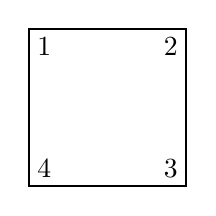
\begin{tikzpicture}
		\node[draw=black, thick,minimum width=2cm,minimum height=2cm] (rect) at (0,0) {};
		\foreach \anc/\n in {south west/4,north west/1,north east/2,south east/3}{
			\node[anchor=\anc] at (rect.\anc) {\n};
		}
	\end{tikzpicture}
	\end{equation*}
	Now, there are four rotations of this square about its center, resulting in the permutations (falling to the shorter notation) $(1\;2\;3\;4), (2\;3\;4\;1), (3\;4\;1\;2), (4\;1\;2\;3)$. There are two reflections about a line passing through the center and one of the vertices (as if the line passes through one vertex, it also passes by the one directly across the center), those result in the permutations $(1\;4\;3\;2)$ and $(3\;2\;1\;4)$. There are also the two reflections about a line passing through the center and a middle of one of the sides, there we get $(2\;1\;4\;3)$ and $(4\;3\;2\;1)$. But that is all the $8$ symmetries of this square, thus we have a homomorphism $D_8 \to S_4$.
\end{proof}

% Problem 2.5
\begin{problem}
\end{problem}

\begin{solution}
	Let $D_{2n}$ be a dihedral group, i.e. the group of symmetries of a regular polygon with $n$ vertices. Let $x$ be a reflection about the center of the polygon and any vertex. Clearly, it must hold that $x^2 = e$, as reflecting about the same line twice returns all the vertices to their original places. Let $y$ be a counterclockwise rotation by $2\pi/n$. Rotating the polygon $n$ times gives us back the original polygon, and thus $y^n=e$.  Now, notice that composing those two symmetries like $xyxy$ gives us back the original polygon, but then $xyxy=e$ and thus $xy=y^{-1}x^{-1}$ and thus $yxy=x$ (because order of $x$ is $2$). Using this relation we can simplify any product in $D_{2n}$. Suppose $x^{i_1}y^{i_2}x^{i_3}y^{i_4}\dots$ is such a product. The only tricky situation is when $x$ is trailing in the product, but we can easily show that from the relation $yxy=x$, for $y^kx=y^{k+1}xy=\dots=xy^{n-k}$. Thus any product can be simplified to $x^iy^j$ for some $i,j$ with $0 \leq i <2$ and $0 \leq j < n$.
\end{solution}

% Problem 2.6
\begin{problem}
\end{problem}

\begin{solution}
	For the case $n=1$, we can easily take $g=h$, since $\abs{g}=2$, we have $gg=e$ and thus $\abs{gh}=1$ as needed.
	
	Now suppose $n > 1$. Now consider the group $D_{2(n)}$. By Problem II.2.5. there are elements $x,y \in D_{2n}$ such that $\abs{x}=n$, $\abs{y}=2$ and $\abs{xy}=2$. But then $\abs{xyy}=\abs{x}=n$, as needed.
\end{solution}

% Problem 2.7
\begin{problem}
\end{problem}

\begin{solution}
	By Problem II.2.6. any element of $D_{2n}$ can be written as a product $xy^i$ or $y^i$, $0 \leq i < n$. Now, consider the elements of the form $y^i$, $0 < i < n$. For $y^i$ to commute with $x$, we need to have $x y^i=y^i x$ by definition. But $x y^i = x y y^{i-1} = y^{-i} x$ (as $\abs{xy}=2$). But that means $y^i = y^{-i}=(y^i)^{-1}$ and thus $\abs{y^i}=2$. But by Proposition I.1.13. we know that $\abs{y^i}=\frac{\abs{y}}{\gcd(i, \abs{y}}=\frac{n}{\gcd(i,n)}=2$. So in particular $\gcd(i,n)=\frac{n}{2}$. Since $i < n$, it follows that $i=\frac{n}{2}$.
		
	Now consider elements of the form $xy^i$. If such an element commutes with everything, it has to commute with $x$ in particular. We have $xxy^i=y^i$ and $xy^ix=x^2y^{-i}=y^{-i}$. Now this can only happen for $i = \frac{n}{2}$. Now, it must also commute with $y$. We have $yxy^i=xy^{i-1}$ and $xy^{i}y=xy^{i+1}$. Now, $xy^{i-1}=xy^{i+1}$ would mean $y^{i-1}=y^{i+1}$, which in turn would mean $y^2=e$. But that only happens if $n=2$.
	
	Therefore we have found that there are no elements that commute with everything for groups $D_{2n}$ where $n$ is odd. In the case $n=2$, $y$ and $xy$ commute with everything. In the case $n > 2$, the only element is $y^{\frac{n}{2}}$.
\end{solution}

% Problem 2.8
\begin{problem}
\end{problem}

\begin{solution}
	[not interested]
\end{solution}

% Problem 2.9
\begin{problem}
\end{problem}

\begin{solution}
	Let $n\in\mathbb{N}$ and $\equiv$ be the 'congruence modulo $n$' relation. Now, let $a,b,c \in \mathbb{Z}$ be numbers. We will prove that $\equiv$ is an equivalence relation:
	\begin{itemize}
		\item We have $a-a=0$ and trivially $n | 0$, thus $a \equiv a$.
		\item Suppose $a \equiv b$. Then $n | (b - a)$ by definition. But then there is $k \in \mathbb{Z}$ such that $(b - a) = kn$. But then $-(b - a) = (a - b) = -kn$, and that means $n | (a - b)$. Therefore $b \equiv a$.
		\item Suppose $a \equiv b$ and $b \equiv c$. Then we have $n | (b - a)$ and $n | (c - b)$. But then there are $k,l \in \mathbb{Z}$ such that $(b - a) = kn$ and $(c - b) = ln$. Summing those two equations we obtain $(b - a) + (c - b) = (c - a) = kn + ln = (k + l)n$ and thus $a \equiv c$.
	\end{itemize}
\end{solution}

% Problem 2.10
\begin{problem}
\end{problem}

\begin{solution}
	Let $\mathbb{Z}/n\mathbb{Z}$ be a cyclic group. The group is the set of equivalence classes of congruence modulo $n$ on $\mathbb{Z}$. Clearly, the $n$ elements $[0]_n,[1]_n,\dots,[n-1]_n$ are all distinct, as if we had $[i]_n = [j]_n$, $0 \leq i < j < n$ (clearly it does not matter if $i < j$ or $j < i$), then $i \equiv j$ so $n | (j - i)$ and thus $j - i = kn$ for some $k \in \mathbb{Z}$. But that is a contradiction, as $i < j < n$ so $j - i < n$ and $i \neq j$ so $j - i \neq 0$.
	
	Now, let $m \in \mathbb{Z}$ be a number such that $m < 0$ or $n \leq m$. Then we can divide $m$ by $n$ such that we get $n = km + i$ for some $k \in \mathbb{Z}$ and $0 \leq i < n$. But that means $n | (m - i)$ and thus $m \equiv i$ and therefore $[m]_n = [i]_n$.
	
	Thus, there are precisely $n$ elements of $\mathbb{Z}/n\mathbb{Z}$ given above.
\end{solution}

% Problem 2.11
\begin{problem}
\end{problem}

\begin{solution}
	Let $n \in \mathbb{Z}$ be an odd integer. Then we can write $n=2k+1$ for some $k \in \mathbb{Z}$ by the definition of an odd integer. Then we have $n^2=(2k+1)^2=4k^2+4k+1$. Now, there are two possibilities, either $k$ is even, or $k$ is odd.
	
	Suppose $k$ is even, then $k = 2l$ for some $l \in \mathbb{Z}$. But then $n^2=16l^2+8l+1$, which means $8 | n^2-1$, so that $n \equiv 1 \mod 8$.
	
	Now suppose $k$ is odd, then $k=2l+1$ for some $l \in \mathbb{Z}$. Then $n^2=16l^2+16l+4+8l+4+1=16l^2+24l+9$ so that again $8 | n^2 - 1$ and thus $n \equiv 1 \mod 8$.
\end{solution}

% Problem 2.12
\begin{problem}
\end{problem}

\begin{solution}
	If there are some nonzero integers $a, b, c \in \mathbb{Z}$ such that $a^2+b^2=3c^2$, then the equation $[a]^2_4+[b]^2_4=3[c]^2_4$ in $\mathbb{Z}/4\mathbb{Z}$ would also have to hold. Now, notice that for any $n \in \mathbb{Z}$, $[n]^2_4$ can either equal $0$ (if $n$ is even) or $1$ ($n$ odd). Therefore for the equation to hold in $\mathbb{Z}/4\mathbb{Z}$, $a, b, c$ all have to be even. Let $a=2k, b=2l, c=2m$ for some $k,l,m \in \mathbb{Z}$. Then we have $k^2+l^2=3m^2$. But again, $k,l,m$ have to be even. We can continue this process until we reach $1$ for some of the factors, proving that indeed $a^2+b^2=3c^2$ does not have a non trivial solution in $\mathbb{Z}$.
\end{solution}

% Problem 2.13
\begin{problem}
\end{problem}

\begin{solution}
	Suppose that $m,n \in \mathbb{Z}$ are numbers such that $\gcd(m,n) = 1$. Then by Corollary II.2.5. we see that $[m]_n$ is a generator of $\mathbb{Z}/n\mathbb{Z}$. But there is some $a \in \mathbb{Z}$ such that $a[m]_n=[am]_n=[1]_n$. But that means $am \equiv 1 \mod n$, so $n | (am - 1)$, and therefore $(am - 1) = cn$. But that shows exactly what we required, there are $a,b \in \mathbb{Z}$ such that $am - cn = am + bn = 1$.
	
	Conversely, suppose there are integers $a, b$ such that $am+bn=1$. But then $[am+bn]_n=[am]_n=[1]_n$. But then if $[x]_n \in \mathbb{Z}/n\mathbb{Z}$ is any element of the group, we have $[x]_n=x[1]_n=x[am]_n=xa[m]_n$. But that means $[m]_n$ generates the group, and thus by Corollary II.2.5. $\gcd(m,n)=1$ must hold.
\end{solution}

% Problem 2.14
\begin{problem}
\end{problem}

\begin{solution}
	Suppose $a \equiv a' \mod n$ and $b \equiv b' \mod n$. Then we have $n | (a' - a)$ and thus $a' - a = kn$, similarly we have $b' - b = ln$, for some $k,l \in \mathbb{Z}$. Now, $a'b'-ab=a'b'-(a'-kn)(b'-ln)=a'b'-(a'b'-a'ln-b'kn+lkn^2)=(-a'l-b'k+lkn)n$. But then $n | (a'b'-ab)$, so $[ab]_n=[a'b']_n$. But that means that multiplication of equivalence classes is well-defined.
\end{solution}

% Problem 2.15
\begin{problem}
\end{problem}

\begin{solution}
	Let $n > 0$ be an odd integer.
	\begin{itemize}
		\item Let $m$ be an integer and $\gcd(m,n)=1$. By Exercise II.2.13. there are integers $a,b$ such that $am+bn=1$. But then we have $4am+4bn=4am+2n+4bn-2n=2a(2m+n)+2n(2b-a)=4$. But that means that $\gcd(2m+n,2n) | 4$, as it must divide the whole equation. But $2m+n$ is odd, since $n$ is odd. Thus $\gcd(2m+n,2n)=1$.
		\item Now, let $r$ be an integer and suppose $\gcd(r,2n)=1$. Then we have, again by Exercise II.2.13., $ar+b2n=1$ for some integers $a,b$. But then we have $ar+an+b2n-an=a(r+n)+n(2b-a)=2a\frac{r+n}{2}=n(2b-a)=1$. Using the result of Exercise II.2.13. again we get $\gcd(\frac{r+n}{2},n)=1$.
		\item Consider the function $f: (\mathbb{Z}/n\mathbb{Z})^* \to (\mathbb{Z}/2n\mathbb{Z})^*$ defined as $f([m]_n)=[2m+n]_{2n}$. Now, this function is well defined, as if $[m]_n \in (\mathbb{Z}/n\mathbb{Z})^*$ we have $\gcd(m,n)=1$ so $\gcd(2m+n,2n)=1$ and thus $[2m+n]_{2n} \in (\mathbb{Z}/2n\mathbb{Z})^*$. Now, define a function $g: (\mathbb{Z}/2n\mathbb{Z})^* \to (\mathbb{Z}/n\mathbb{Z})^*$ as $g([r]_{2n})=[\frac{r+n}{2}]_n$. This function is again well defined. Now, $gf([m]_n)=g([2m+n]_{2n})=[\frac{2m+2n}{2}]_n=[m+n]_n=[m]_n$ and thus $g$ is an inverse of $f$. But that means $(\mathbb{Z}/n\mathbb{Z})^*$ and $(\mathbb{Z}/2n\mathbb{Z})^*$ are isomorphic.
	\end{itemize}
\end{solution}

% Problem 2.16
\begin{problem}
\end{problem}

\begin{solution}
	To find the last digit of $1238237^{18238456}$ we will work in $\mathbb{Z}/n\mathbb{Z}$. We have $[1238237]_10=[7]_10$. Now $[7^2]_10=[9]_10$, $[7^3]_10=[3]_10$, $[7^4]_10=[1]_10$. But $[18238456]_4=0$, and thus the last digit is $1$.	
\end{solution}

% Problem 2.17
\begin{problem}
\end{problem}

\begin{solution}
	Suppose $m \equiv m' \mod n$. Then $n | (m' - m)$ so $m' - m = kn$ for some integer $k$. Now, suppose that $\gcd(m,n)=1$. Then by Exercise II.2.13. there are integers $a,b$ such that $am+bn=1$. But $m = m' - kn$, so we have $a(m' - kn)+bn=am'-akn+bn=am'+(b-ak)n=1$, and thus $\gcd(m',n)=1$. 
	
	If $\gcd(m',n)=1$, then again there are integers $a,b$ such that $am'+bn=1$. But $m' = kn - m$, so $am'+bn=a(kn - m) + bn=akn-am+bn=(-a)m+(ak+b)n=1$ and thus $\gcd(m,n)=1$.
\end{solution}

% Problem 2.18
\begin{problem}
\end{problem}

\begin{solution}
	Define the function as follows. For $[m]_d$ we move every element up to $d$ $m$ places to the right, wrapping around. This way, $[0]_d$ is the identity permutation, $[1]_d$ is the permutation $(d\;1\;2\;dots\;d-2\;d-1\;d+1\;\dots n)$. Composing this morphism gets us the permutation $(d-1\;d\;1\dots)$ etc. So indeed, those morphisms preserve the structure.
\end{solution}

% Problem 2.19
\begin{problem}
\end{problem}

\begin{solution}
	[do not want to typeset the tables]
\end{solution}

\subsection{The category $\mathsf{Grp}$}

% Problem 3.1
\begin{problem}
\end{problem}

\begin{solution}
	Let $\C$ be a category with products and $\varphi: G \to H$ a morphism in $\C$. Now, if we have products $G \times G$ and $H \times H$ with the corresponding projection morphisms $\pi_G$ and $\pi_H$, we can use the universal property of products as follows: Since $H \times H$ with $\pi_H$ satisfies the universal property, for any object $X$, such that there is a morphism $X \to H$, there is a unique morphism $X \to H \times H$. But notice that for $G \times G$ we have the morphism $\varphi \pi_G: G \times G \to H$ and thus there is a unique morphism (which by uniqueness we can call $\varphi \times \varphi$) such that $\varphi \times \varphi: G \times G \to H \times H$.
\end{solution}

% Problem 3.2
\begin{problem}
\end{problem}

\begin{solution}
	Let $\C$ be a category with products and $\varphi: G \to H$ and $\psi: H \to K$ morphisms in $\C$. By Exercise II.3.1. there are then morphisms $(\varphi \times \varphi): G \times G \to H \times H$ and $(\psi \times \psi): H \times H \to K \times K$. It is also easy to see that $(\psi\varphi) \times (\psi\varphi)$ is the unique morphism $G \times G \to K \times K$. But $(\psi \times \psi)(\varphi \times \varphi): G \times G \to K \times K$ is also such a morhism. Thus by the universal property of products those two morphisms must be isomorphic.
\end{solution}

% Problem 3.3
\begin{problem}
\end{problem}

\begin{solution}
		Suppose $G$ and $H$ are commutative groups. Consider the product of those groups, $G \times H$, with the two natural homomorphisms $i_G: G \to G \times H$ and $i_H: H \to G \times H$. For this construction to satisfy the universal property of coproducts in $\mathsf{Ab}$, for any commutative group $Z$ such that there are morphisms $g: G \to Z$ and $h: H \to Z$, there must be a unique morphism $\sigma: G \times H \to Z$. Diagram-wise it means that there is a morphism $\sigma$ such that the following diagram commutes:
		\begin{equation*}
			\begin{tikzcd}
				G
					\arrow[drr, bend left, "g"]
					\arrow[dr, "i_G" swap]
					& &\\
				&
					G \times H
						\arrow[r, "\sigma"]
					& Z\\
				H
					\arrow[urr, bend right, "h" swap]
					\arrow[ur, "i_H"]
					& &
			\end{tikzcd}
		\end{equation*}
		Now, the only choice for $\sigma$ is given by the set-function $\sigma((a,b))=g(a)h(b)$. We have to check that $\sigma$ is a group homomorphism. $\sigma((a,b)(c,d))=\sigma((ac,bd))=g(ac)h(bd)=g(a)g(c)h(b)h(d)=g(a)h(b)g(c)h(d)=\sigma((a,b))\sigma((c,d))$, precisely because $Z$ is commutative. Therefore, $G \times H$ satisfies the universal propery of coproducts in $\C$.
\end{solution}

% Problem 3.4
\begin{problem}
\end{problem}

\begin{solution}
	$H$ does not necesarrily have to be the trivial group. One example is $R$ and $R \times R$, as additive groups. The process of finding the explicit bijection is beyond the scope of algebra though.
\end{solution}

% Problem 3.5
\begin{problem}
\end{problem}

\begin{solution}
	Let $\mathbb{Q}=G \times H$. If both $G, H$ is trivial, then $\mathbb{Q}$ would be trivial, and thus, without loss of generality, say that $G$ is non-trivial. Now, consider the canonical projection $\pi_G$. By its definition, $\pi_G((e_G,h))=e_G$ for all $h \in H$.
	
	Suppose $m \neq 0$ and $g \in G$, with $mg=0_G$. But then we have $m(g,e_H)=e_{G \times H}$. But $\mathbb{Q}$ has no non-zero elements of finite order, so we must have $g = e_G$.
	
	Now, suppose that for some $n \neq 0$ and $m \neq 0$ we have $\pi_G(\frac{n}{m})=e_G$. Then we have $m \pi_G(\frac{n}{m}) = \pi_G(n) = n \pi_G(1) = e_G$. But that means $\pi_G(1) = e_G$. Since $1$ generates $\mathbb{Z}$, this means $\pi_G$ maps every integer to $e_G$.
	
	Now let $a, b$ be any integers such that $a \neq 0$ and $b \neq 0$. We have $b \pi_G(\frac{a}{b}) = \pi_G(a) = e_G$. But that means, again that $\pi_G(\frac{a}{b}) = e_G$.
	
	Now, suppose there is an element $(e_G, h)$ such that $h \neq e_H$. But $\pi_G(e_G, h) = e_G$ by the definition of the natural projection, so $\pi_G$ must necessarily map everything to $e_G$. But $G$ is non-trivial, and therefore $H$ must be trivial. 
\end{solution}

% Problem 3.6
\begin{problem}
\end{problem}

\begin{solution}
	Going point by point:
	\begin{itemize}
		\item Let $f: C_2 \to S_3$ be defined as $f(e) = (1\;2\;3)$ and $f(x) = (2\;1\;3)$. Then $f(x^n)=e$ if $2 | n$ or $f(x^n)=(2\;1\;3)$ otherwise. Thus this is an injective homomorphism. Now, let $g: C_3 \to S_3$ be defined as $g(e)=(1\;2\;3)$, $g(x)=(2\;3\;1)$ and $g(x^2)=(3\;1\;2)$. Now, $g(x)g(x)=(3\;1\;2)=g(x^2)$, and $g(x)g(x^2)=(1\;2\;3)$, so it is indeed an injective homomorphism.
		\item Suppose $C_2 \times C_3$ is the coproduct of $C_2$ and $C_3$ in $\mathsf{Grp}$. By the universal property of coproducts,  as there are morphisms $C_2 \to S_3$ and $C_3 \to S_3$, this means there is a unique homomorphism $\sigma: C_2 \times C_3 \to S_3$, such that $\sigma i_{C_2} = f$ and $\sigma i_{C_3} = g$.
		\item Now, notice that $i_{C_2}$ must necessarily map an element $x \in C_2$ to $(x, e_{C_3})$, and similarly for $i_{C_3}$. But then we have $f(x_1)g(x_2)=\sigma((x_1, e_{C_3})(e_{C_2}, x_2))=\sigma((x_1, x_2))=\sigma((e_{C_2}, x_2)(x_1, e_{C_3})=g(x_2)f(x_1)$. But we have, for example, $(2\;1\;3)(2\;3\;1)=(3\;2\;1)$ and $(2\;3\;1)(2\;1\;3)=(1\;3\;2)$. Thus $\sigma$ cannot exist (precisely because $S_3$ is not commutative).
	\end{itemize}
\end{solution}

% Problem 3.7
\begin{problem}
\end{problem}

\begin{solution}
	TODO
\end{solution}

% Problem 3.8
\begin{problem}
\end{problem}

\begin{solution}
	Define a group $G$ as the group generated by two elements $x, y$ such that $x^2=e_G$ and $y^3=e_G$. Then we can define group homomorphisms $i_{C_2}: C_2 \to G$ and $i_{C_3}: C_3 \to G$ as follows: $i_{C_2}(e_{C_2})=e_G$, $i_{C_2}(c_2)=x$, $i_{C_3}(e_{C_3})=e_G$, $i_{C_3}(c_3)=y$, $i_{C_3}(c_3^2)=y^2$.
	
	Now, suppose $Z$ is any group, and $f: C_2 \to Z$ and $g: C_3 \to Z$ group homomorphisms. Now, by the universal property of coproducts in $\mathsf{Grp}$ we require to construct a group homomorphism $\sigma$, such that $\sigma i_{C_2} = f$ and $\sigma i_{C_3} = g$. But because any element $z$ of $G$ is generated by $x$ and $y$, we must have $\sigma(x) = f(c_2)$ and $\sigma(y) = g(c_3)$ and this is enough for the definition, because $z$ can be written as a product of $x$ and $y$.
\end{solution}

% Problem 3.9
\begin{problem}
\end{problem}

\begin{solution}
	The definition of the fiber product is pretty straightforward, and follows straight from the definition for $\mathsf{Set}$. We only have to check that the definition satisfies the group axioms and satisfies the required universal property. Let $A,B,C$ be groups and $\alpha: A \to C$, $\beta: B \to C$ group homomorphisms. Define $A \times_C B = \set{(a,b) \in A \times B \mid \alpha(a)=\beta(b)}$.
	
	To check that this construction is a group, we will take the operation to be the same as the one on $A \times B$, i.e. $(a,b)(c,d)=(ac,bd)$. This operation is well-defined, as we have $\alpha(a)=\beta(b)$ and $\alpha(c)=\beta(d)$, and since $\alpha, \beta$ are group homomorphisms, $\alpha{ab}=\alpha(a)\alpha{b}=\beta{c}\beta{d}=\beta{cd}$. Now, we have to prove that $(e_A, e_B)$ is an element of the group. But we have $\alpha(e_A)=e_C=\beta(e_B)$, again because they are homomorphisms. Now, suppose $(a,b) \in A \times_C B$. Then $\alpha(a)=\beta(b)$, so $(\alpha(a))^{-1}=(\beta(b))^{-1})$ and again because they are homomorphisms, $\alpha(a^{-1})=\beta(b^{-1})$. Therefore $(a^{-1}, b^{-1}) \in A \times_C B$, but that is an inverse of $(a, b)$. Thus $A \times_C B$ is a group.
	
	Now, we have to prove that this construction satisfies the universal property of a fiber product. Suppose $Z$ is a group and $f, g$ the respective homomorphisms, such that $\alpha f = \beta g$. To ensure the commutativity of the respective diagram, we have to define $\sigma: Z \to A \times_C B$ as follows: $\sigma(z)=(f(z),g(z))$.  It is well defined, as we have $(\alpha f)(z) = (\beta g)(z)$, so $\alpha (f(z))=\beta(g(z))$. To see that this is a group homomorphism, note that $\sigma(z_1 z_2) = (f(z_1z_2), g(z_1z_2)) = (f(z_1)f(z_2),g(z_1)g(z_2))=(f(z_1), g(z_1))(f(z_2), g(z_2))=\sigma(z_1)\sigma(z_2)$.

	The commutativity of the diagram follows from the definition easily, note that we have $(\pi_A \sigma)(z)=\pi_A(\sigma(z))=\pi_A((f(z), g(z)))=f(z)$ so $\alpha \pi_A \sigma = \alpha f$ and similarly for the other side of the diagram.
	
	To define the fibered coproduct in $\mathsf{Ab}$ we require knowledge of quotients, which have to yet been introduced.
\end{solution}

\subsection{Group homomorphisms}

% Problem 4.1
\begin{problem}
\end{problem}

\begin{solution}
	Suppose $m | n$ and $a \cong a' \mod n$. Then $n | (a' - a)$. But then $m | (a' - a)$, and thus $[a]_m = [a']_m$.
	
	To check it makes the diagram commute, notice that for any $z \in \mathbb{Z}$ we have $(\pi^n_m \pi_n)(z)=\pi^n_m([z]_n)=[z]_m=\pi_m(z)$ by the definition of the function.
	
	To verify it is indeed a group homomorphism, let $a,b$ be elements of $\mathbb{Z}_n$. Then we have $\pi^n_m(a+b)=[a+b]_m=[a]_m + [b]_m = \pi^n_m(a) + \pi^n_m(b)$.
	
	Thus $\pi^n_m$ is a well-defined group homomorphism that makes the diagram commute. The hypothesis $m | n$ is necessary as the order of all elements of $\mathbb{Z}_n$ divides $n$ and the order of all elements of $\mathbb{Z}_m$ divides $m$, and it also must hold that $\abs{\pi^n_m(z)} \mid \abs{z} \mid n$. Now if $m \nmid n$, then $\pi^n_m([1]_n)=[1]_m$ but $\abs{\pi^n_m([1]_n)}=m \nmid n$, a contradiction.
\end{solution}

% Problem 4.2
\begin{problem}
\end{problem}

\begin{solution}
	The homorphim is defined pretty explicitly so we can easily check that the image of the homomorphism is the set $\set{(0,0),(1,1)}$, which is not isomorphic to $C_2 \times C_2$. We can actually show that there is no such isomophism. Suppose $f: C_4 \to C_2 \times C_2$ is an isomorphism of groups. Because $C_4$ is cyclic, we have $f([0]_4)=([0]_2,[0]_2)$, $f([2]_4])=2f([1]_4)$ and $f([3]_4)=3f([1]_4)$. But is in truth a contradiction to our assumption of isomorphism, as there are three reasonable choices for $f([1]_4)$, but choosing any of those breaks isomorphism.
\end{solution}

% Problem 4.3
\begin{problem}
\end{problem}

\begin{solution}
	Suppose $G$ is a group of order $n$ isomorphic to $\mathbb{Z}/n\mathbb{Z}$. Let $\varphi: \Z{n} \to G$ be a group isomorphism. There is an element of order $n$ in $\Z{n}$, namely $[1]_n$. By Proposition II.4.8. $\abs{\varphi([1]_n)}=\abs{[1]_n}=n$, thus $G$ contains an element of order $n$.
	
	Suppose the converse holds, i.e. $G$ is a group of order $n$ which contains an element $x$ of 
	order $n$. Because $x$ has order $n$, the elements $x^0, x^1, \dots, x^{n-1}$ must make up all of 
	G. We can easily define an isomorphism $\rho: G \to \Z{n}$ for $g \in G$ by finding the unique index 
	$i$ for which $g = x^i$ and setting $\rho(g) = [i]_n$. The proof of $\rho$ being an isomorphism is 
	mechanical.
\end{solution}

\end{document}